%%%%%%%%%%%%%%%%%%%%%%%%%%%%%%%%%%%%%%%%%%%%%%%%%%%%%%%%%%%%%%%%%%%%%%%%%%%%%%%%%%%%%%%
%%%%%%%%%%%%%%%%%%%%%%%%%%%%%%%%%%%%%%%%%%%%%%%%%%%%%%%%%%%%%%%%%%%%%%%%%%%%%%%%%%%%%%%
% 
% This top part of the document is called the 'preamble'.  Modify it with caution!
%
% The real document starts below where it says 'The main document starts here'.

\documentclass[12pt]{article}
\usepackage{graphicx}
\usepackage{float}
\usepackage{amssymb,amsmath,amsthm}
\usepackage[top=1in, bottom=1in, left=1.25in, right=1.25in]{geometry}
\usepackage{fancyhdr}
\usepackage{enumerate}

% Comment the following line to use TeX's default font of Computer Modern.
\usepackage{times,txfonts}

\newtheoremstyle{homework}% name of the style to be used
  {18pt}% measure of space to leave above the theorem. E.g.: 3pt
  {12pt}% measure of space to leave below the theorem. E.g.: 3pt
  {}% name of font to use in the body of the theorem
  {}% measure of space to indent
  {\bfseries}% name of head font
  {:}% punctuation between head and body
  {2ex}% space after theorem head; " " = normal interword space
  {}% Manually specify head
\theoremstyle{homework} 

% Set up an Exercise environment and a Solution label.
\newtheorem*{exercisecore}{Exercise \@currentlabel}
\newenvironment{exercise}[1]
{\def\@currentlabel{#1}\exercisecore}
{\endexercisecore}

\newcommand{\localhead}[1]{\par\smallskip\noindent\textbf{#1}\nobreak\\}%
\newcommand\solution{\localhead{Solution:}}

%%%%%%%%%%%%%%%%%%%%%%%%%%%%%%%%%%%%%%%%%%%%%%%%%%%%%%%%%%%%%%%%%%%%%%%%
%
% Stuff for getting the name/document date/title across the header
\makeatletter
\RequirePackage{fancyhdr}
\pagestyle{fancy}
\fancyfoot[C]{\ifnum \value{page} > 1\relax\thepage\fi}
\fancyhead[L]{\ifx\@doclabel\@empty\else\@doclabel\fi}
\fancyhead[C]{\ifx\@docdate\@empty\else\@docdate\fi}
\fancyhead[R]{\ifx\@docauthor\@empty\else\@docauthor\fi}
\headheight 15pt

\def\doclabel#1{\gdef\@doclabel{#1}}
\doclabel{Use {\tt\textbackslash doclabel\{MY LABEL\}}.}
\def\docdate#1{\gdef\@docdate{#1}}
\docdate{Use {\tt\textbackslash docdate\{MY DATE\}}.}
\def\docauthor#1{\gdef\@docauthor{#1}}
\docauthor{Use {\tt\textbackslash docauthor\{MY NAME\}}.}
\makeatother

% Shortcuts for blackboard bold number sets (reals, integers, etc.)
\newcommand{\Reals}{\ensuremath{\mathbb R}}
\newcommand{\Nats}{\ensuremath{\mathbb N}}
\newcommand{\Ints}{\ensuremath{\mathbb Z}}
\newcommand{\Rats}{\ensuremath{\mathbb Q}}
\newcommand{\Cplx}{\ensuremath{\mathbb C}}
%% Some equivalents that some people may prefer.
\let\RR\Reals
\let\NN\Nats
\let\II\Ints
\let\CC\Cplx

%%%%%%%%%%%%%%%%%%%%%%%%%%%%%%%%%%%%%%%%%%%%%%%%%%%%%%%%%%%%%%%%%%%%%%%%%%%%%%%%%%%%%%%
%%%%%%%%%%%%%%%%%%%%%%%%%%%%%%%%%%%%%%%%%%%%%%%%%%%%%%%%%%%%%%%%%%%%%%%%%%%%%%%%%%%%%%%
% 
% The main document start here.

% The following commands set up the material that appears in the header.
\doclabel{Stat 300: Homework 4}
\docauthor{Stefano Fochesatto}
\docdate{\today}

\begin{document}
\begin{enumerate}



\item\hspace{.5in}\textbf{Exercise 3.30:} An individual who has automobile insurance from a certain company is randomly selected. Let $Y$ be the number of moving violations for which the individual was cited during the last $3$ years. The $pmf$ of $Y$ is,
\begin{center}
  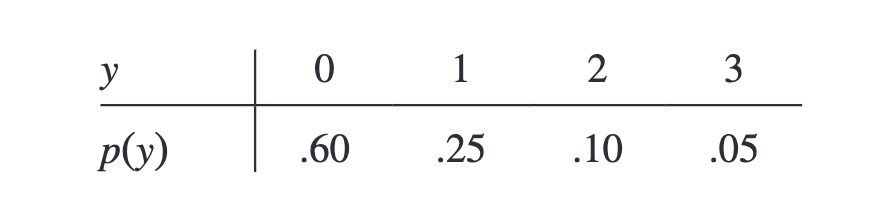
\includegraphics[width = .50\textwidth]{pmf.png}
\end{center}
\begin{enumerate}
\item Compute $E(Y)$.
\item Suppose an individual with $Y$ violations incurs a
surcharge of $\$100Y^2$ . Calculate the expected amount
of the surcharge.
\end{enumerate}

\textbf{Answer:} 
\begin{enumerate}
\item To calculate the expected value we have to sum the support multiplied by the corresponding value of the $pmf$.
therefore,
\begin{equation*}
  E(Y) = \sum_{y = 0}^3 yp(y) = 0(.60) + 1(.25) + 2(.10) + 3(.05) = .60
\end{equation*}
\item To calculate the expected value of $h(Y) = 100Y^2$ we use,
\begin{equation*}
  E(100Y^2) = \sum_{y = 0}^3 h(y)p(y) = (100) 0^2(.60) + (100) 1^2(.25) + (100) 2^2(.10) + (100) 3^2(.05) = 110
\end{equation*}
\end{enumerate}

\vspace{.5in}





\item\hspace{.5in}\textbf{Exercise 3.34:} Suppose that the number of plants of a particular type found in a rectangular sampling region (called a quadrat by ecologists) in a certain geographic area is an $rv$ $X$ with $pmf$,
\begin{center}
  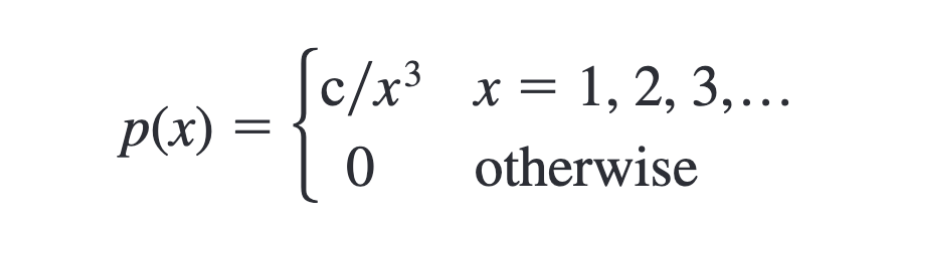
\includegraphics[width = .50\textwidth]{pmf2.png}
\end{center}
\begin{enumerate}
\item Is E(X) finite? Justify your answer (this is another distribution that statisticians would call heavy-tailed).\\
\end{enumerate}
\textbf{Answer:} 

\begin{enumerate}
  \item Consider the expected value, calcuated with an infinite sum,
  \begin{equation*}
    \sum_{i = 1}^{\infty}xp(x) = c\sum_{i = 1}^{\infty}\dfrac{1}{x^2}.
  \end{equation*}
  Since the infinte series,
  \begin{equation*}
    \sum_{i = 1}^{\infty}\dfrac{1}{x^2},
  \end{equation*}
  is convergent we know that the excpected value exists. 
\end{enumerate}
\vspace{.5in}







\item\hspace{.5in}\textbf{Exercise 3.48:} NBC News reported on May 2, 2013, that $1$ in $20$ children in the United States have a food allergy of some sort. Consider selecting a random sample of $25$ children and let $X$ be the number in the sample who have a food allergy. Then $X\sim Bin(25, .05)$.
\begin{enumerate}
\item Determine both $P(X \le 3)$ and $P(X < 3)$.
\item Determine $P(X \ge 4)$.
\item Determine $P(1 \le X \le 3)$.
\item What are $E(X)$ and $\sigma_X$?
\item In a sample of $50$ children, what is the probability that none has a food allergy?
\end{enumerate}

\textbf{Answer:} 
\begin{enumerate}
\item Consider the following equation,
\begin{equation*}
  P(X \le 3) = \sum_{i = 0}^{3}p(i)
\end{equation*}
Evaluating the equation with a binomial random variable $X\sim Bin(25, .05)$,
\begin{align*}
  P(X \le 3) &=\binom{25}{0}(.05)^0(.95)^25+\binom{25}{1}(.05)^1(.95)^24+\binom{25}{2}(.05)^2(.95)^23+\binom{25}{3}(.05)^3(.95)^22\\
  &=.966
\end{align*} 
Calculating $P(X < 3) = P(X \le 2)$ so,
\begin{align*}
  P(X \le 2) &= \binom{25}{0}(.05)^0(.95)^25+\binom{25}{1}(.05)^1(.95)^24+\binom{25}{2}(.05)^2(.95)^23\\
  &=.873.
\end{align*}

\item First we will simplify the probability,
\begin{equation*}
  P(X \geq 4) = 1 - P(X < 4) = 1 - P(X \le 3).
\end{equation*}
using our previuos result we get,
\begin{equation*}
  P(X \geq 4) = 1 - .966 = .034
\end{equation*}

\item Again we simplify the probability statement, 
\begin{equation*}
  P(1\le X \le 3) = P(X \le 3) - P(X < 1) = P(X \le 3) - P(X \le 0) 
\end{equation*}
Using our previous results,
\begin{equation*}
  P(1\le X \le 3) = .966 -  \binom{25}{0}(.05)^0(.95)^25 = .689.
\end{equation*}
\item Since $X$ is a binomial random variable we know that $E(X) = 25(.05) = 1.25$ and $\sigma_X = \sqrt{25(.95)(.05)} = 1.0897$
\item Defining a new random variable $X\sim Bin(50, .05)$ and calculating the probability, 
\begin{equation*}
  \binom{50}{0}(.05)^0(.95)^50 = .0769.
\end{equation*}
\end{enumerate}
\vspace{.5in}







\item\hspace{.5in}\textbf{Exercise 3.56:} The College Board reports that $2\%$ of the $2$ million high school students who take the SAT each year receive special accommodations because of documented disabilities \emph{(Los Angeles Times, July 16, 2002)}. Consider a random sample of $25$ students who have recently taken the test.
\begin{enumerate}
\item What is the probability that exactly 1 received a special accommodation?
\item What is the probability that at least 1 received a special accommodation?
\addtocounter{enumii}{1}
\item What is the probability that the number among the $25$ who received a special accommodation is within $2$ standard deviations of the number you would expect to be accommodated?
\end{enumerate}

\textbf{Answer:} 
\begin{enumerate}
\item Consider the binomial random variable $X\sim Bin(25, .02)$ since we have a sample of $25$ student and only 2\% of the population is a success. Therefore the probability that only one will revive accomidations,
\begin{equation*}
 P(X = 1) = {25 \choose 1}(.02)(.98)^{24}=.308
\end{equation*}





\item The probablity of at least one student reciving special accomidation can be calculated by simply taking the compliment,
\begin{equation*}
  1-P(X = 0) = 1-{25 \choose 0}(.02)^0(.98)^{25}=.397
\end{equation*}
\addtocounter{enumii}{1}



\item First we have to calculate the expected value, and standard deviation,
\begin{equation*}
  E(X) = 25(.02).5,\sigma_X = \sqrt(25(.02)(.98)) = .7
\end{equation*}
Then calculating the probability that the nunber among the 25 who recieve special accomidation is within 2 standard deviations is,
\begin{equation*}
  P(.5 - 1.4\le X \le .5 + 1.4) = P(0 \le X \le 1) = {25 \choose 0}(.02)^0(.98)^{25} - {25 \choose 1}(.02)(.98)^{24} = .70443
\end{equation*}
\end{enumerate}
\vspace{.5in}







\item\hspace{.5in}\textbf{Exercise 3.58:} A very large batch of components has arrived at a distributor. The batch can be characterized as acceptable only if the proportion of defective components is at most $.10$. The distributor decides to randomly select $10$ components and to accept the batch only if the number of defective components in the sample is at most $2$.
\begin{enumerate}
\item What is the probability that the batch will be accepted when the actual proportion of defectives is $.01$? $.05$? $.10$? $.20$? $.25$?
\item Let p denote the actual proportion of defectives in the batch. A graph of $P$(batch is accepted) as a function of $p$, with $p$ on the horizontal axis and $P$(batch is accepted) on the vertical axis, is called the operating characteristic curve for the acceptance sampling plan. Use the results of part $(a)$ to sketch this curve for $0 \le p \le 1$.
\item Repeat parts $(a)$ and $(b)$ with “$1$” replacing “$2$” in the acceptance sampling plan.
\end{enumerate}
\textbf{Answer:} 
\begin{enumerate}
\item Consider random variable $X\sim Binom(10,p)$ and Using Appendix A.1 we will calculate $P(X \le 2)$ for the following value of $p$\\

$ p = .01$, $P(X\le 2)=.999$\\
$ p = .05$, $P(X\le 2)=.988$\\
$ p = .10$, $P(X\le 2)=.930$\\
$ p = .20$, $P(X\le 2)=.678$\\
$ p = .25$, $P(X\le 2)=.526$\\
\item Consider the following plot made in $R$,
\begin{center}
  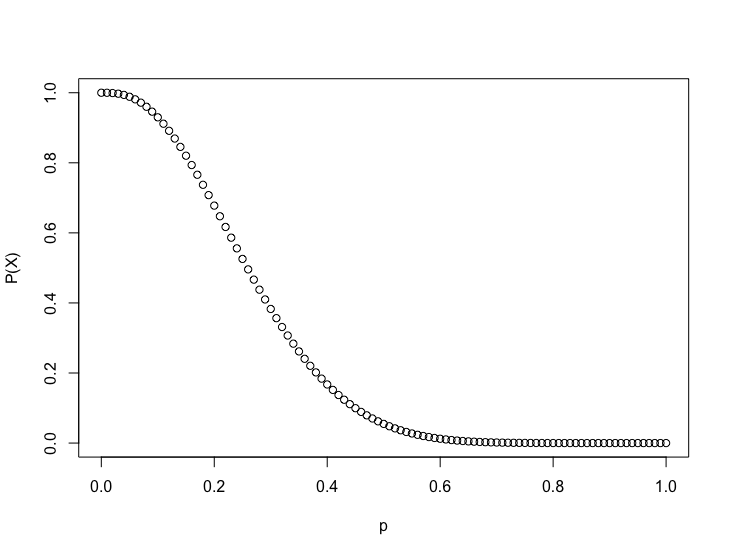
\includegraphics[width = \textwidth]{Rplot.png}
\end{center}



\item Consider random variable $X\sim Binom(10,p)$ and Using Appendix A.1 we will calculate $P(X \le 1)$ for the following value of $p$\\

$ p = .01$, $P(X\le 1)=.996$.\\
$ p = .05$, $P(X\le 1)=.914$.\\
$ p = .10$, $P(X\le 1)=.736$.\\
$ p = .20$, $P(X\le 1)=.376$.\\
$ p = .25$, $P(X\le 1)=.244$.\\
$ p = .50$, $P(X\le 1)=.011$.\\
$ p = .75$, $P(X\le 1)=.00003$.\\

\end{enumerate}
\vspace{.5in}








\item\hspace{.5in}\textbf{Exercise 3.60:} A toll bridge charges $\$1.00$ for passenger cars and $\$2.50$ for other vehicles. Suppose that during daytime hours, $60\%$ of all vehicles are passenger cars. If $25$ vehicles cross the bridge during a particular daytime period, what is the resulting expected toll revenue? [Hint: Let $X= $ the number of passenger cars; then the toll revenue $h(X)$ is a linear function of $X$.]\\
\\
\textbf{Answer:} \\
Consider that the expected value for the random variable, $X \sim (25, .6)$ where the linear funciton that estimates toll revinue is ,
\begin{equation*}
  h(X) = (1)X+(2.5)(25 - X)
\end{equation*}
Therefore using the fact that the expected value is $E(X) = 25(.6)$ we get the expected toll revenue is,
\begin{equation*}
  E((1)X+(2.5)(25 - X)) = E(X)+(2.5)E(25 - X) = 15 + 2.5(10) = 40 
\end{equation*}
\vspace{.5in}

\item\hspace{.5in}\textbf{Supplemental 1:} Suppose that we get $100$ pairs of patients and want to compare two treatments (this is called a matched pairs design).\\

We will apply one treatment to one patient in a pair and the other treatment to the other patient in a pair (random selection within pairs).\\

If both treatments work equally well, the number of pairs where treatment one is better than treatment two should be $X \sim Binomial(100,0.5)$, because in this case it’s essentially a coin flip. What is the expected value and standard deviation of $X$? What range of values is within $2$ standard deviations of the mean?\\
\\
\textbf{Answer:} 
It is known that the mean and standard deviation of a binomialy distributed  random variable are,
\begin{equation*}
  E(X) = np = 100(.5) = 50
\end{equation*}
\begin{equation*}
  \sigma_X = \sqrt{np(1-p)} = 5
\end{equation*}
Calculating the probability within 2 standard deviations from the expected value (r assisted),
\begin{equation*}
  P(40\le X \le 60) = P(X \le 60) - P(X \le 39) = .9647
\end{equation*}
\vspace{.5in}

\item\hspace{.5in}\textbf{Exercise 3.62:}
\begin{enumerate}
\item For fixed $n$, are there values of $p(0 \le p \le 1)$ for which $V(X) = 0$? Explain why this is so.
\item For what value of $p$ is $V(X)$ maximized? [Hint: Either graph $V(X)$ as a function of $p$ or else take a derivative.]
\end{enumerate}
\textbf{Answer:} 
\begin{enumerate}
\item For binomial distributions it is know that we can calculate the variance with the formula,
\begin{equation*}
  V(X) = np(1 - p)
\end{equation*}
Solving this equation for roots where $n$ is a non zero constant and $0 \le p \le 1$ we know that those value of $p$ are the edge cases $p = 1$ and $p = 0$. This makes seance in application since 
it means that an event is certain to happen or impossible to happen and therefore there should be no varice in our probabilities.\\


\item Like the hint suggests we can take the derivative of the previous equation,
\begin{equation*}
  V'(X) = n - 2np = n(1-2p),
\end{equation*}
and clearly we have a root at $p = \frac{1}{2}$ coressponding with the maxima of $V(X)$
\end{enumerate}
\vspace{.5in}

\end{enumerate}
\end{document}